%%=====================================================================================
%%
%%       Filename:  simple_bistable_switch.tex
%%
%%    Description:  
%%
%%        Version:  1.0
%%        Created:  08/03/2016
%%       Revision:  none
%%
%%         Author:  Dilawar Singh (), dilawars@ncbs.res.in
%%   Organization:  NCBS Bangalore
%%      Copyright:  Copyright (c) 2016, Dilawar Singh
%%
%%          Notes:  
%%                
%%=====================================================================================

\RequirePackage{luatex85}
\documentclass[crop,tikz]{standalone}
\usetikzlibrary{positioning,calc,arrows,arrows.meta}
\usepackage{pgfplots}

\begin{document}

\begin{figure}[h!]
\centering
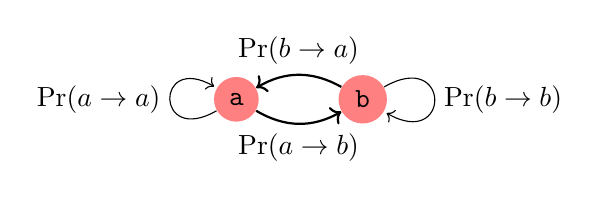
\begin{tikzpicture}[scale=1 , every node/.style={} ]

    \node[] (origin) at (0,0) {};

    \node[circle,fill=red!50] (low) at (origin) {\tt a};
    \node[circle,fill=red!50] (high) [right=of low] {\tt b};

    \draw[->, thick] (low) edge[ bend right] node[below] {$\Pr(a \rightarrow b)$} (high);
    \draw[->, thick] (high) edge[ bend right] node[above] {$\Pr(b \rightarrow a)$} (low);

    \draw[->] (low) edge [in=150,out=210,loop] node[left] {$\Pr(a\rightarrow a)$} (low) ;
    \draw[->] (high) edge [in=-30,out=30,loop] node[right] {$\Pr(b \rightarrow b)$} (high);
    
\end{tikzpicture}	 %
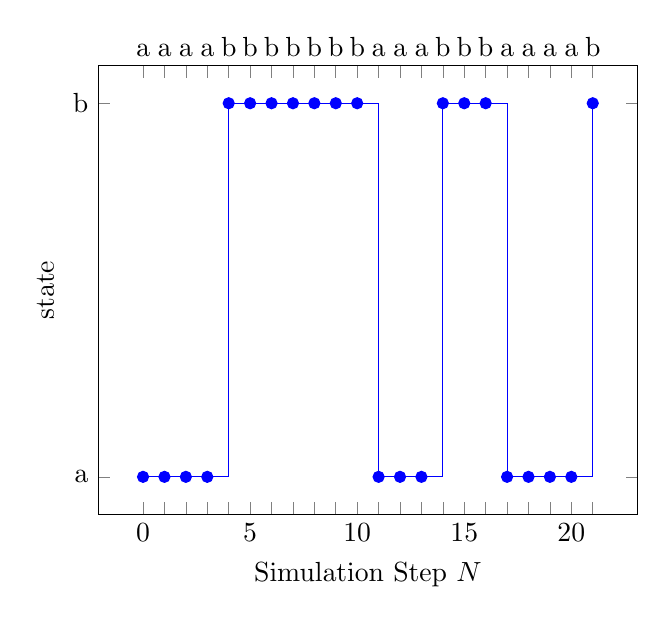
\begin{tikzpicture}
    \begin{axis}[
            xlabel=Simulation Step $N$
            , ylabel=state
            , ytick={0,1}
            , yticklabels = {a, b}
            , extra x ticks = {0,...,21}
            , extra x tick labels = {a,a,a,a,b,b,b,b,b,b,b,a,a,a,b,b,b,a,a,a,a,b}
            , extra x tick style = { ticklabel pos = top }
            %, domain = 0:20
            %, samples = 40
        ]

        %\addplot[mark=*,color=blue,const plot] shell [] { 
                %awk 'BEGIN{
                    %for(i=0;i<100;i++) print i, rand(); }'
            %};
        \addplot[const plot, mark=*, color=blue] coordinates { 
                (0,0) (1,0) (2,0) (3,0) (4, 1)
                (5,1) (6,1) (7,1) (8,1) (9, 1)
                (10,1) (11,0) (12,0) (13, 0) (14, 1)
                (15,1) (16,1) (17,0) (18,0) (19,0) 
                (20, 0) (21, 1)
        };
    \end{axis}
\end{tikzpicture} 

\caption{Typical state transition in a bistable switch.  Each edge shows a
transition with non-zero probability.  {\bf On left} State transition diagram of
a bistable switch. {\bf On right} a realization of such a bistable.  }

\label{fig:typical_bistable_switch}
\end{figure}


\end{document}

